\paragraph{Conclusions} \mbox{}\\[\paragraphheaderspace]
\begin{center}
	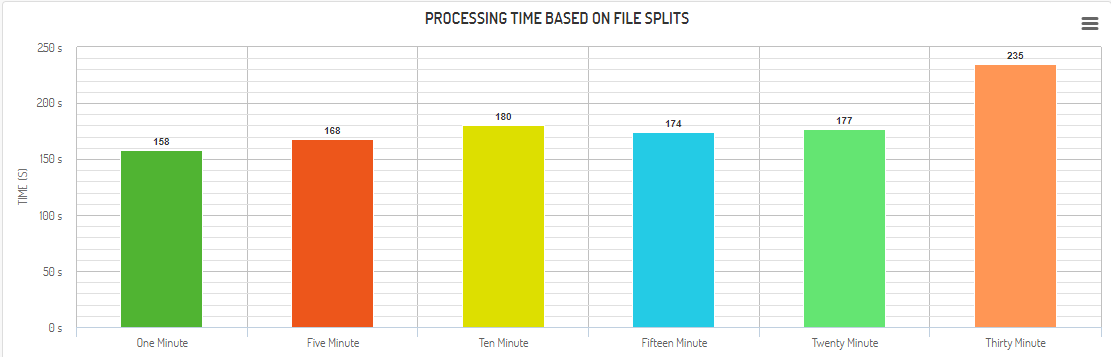
\includegraphics[width=\textwidth]{fileSplits}
\end{center}
Interestingly, all the different splits performed mostly the same \textit{except} for the thirty minute splits. Further, the ten minute splits ended up a tad bit higher than even the fifteen and twenty minute splits. The lowest recorded time was the one minute splits, and the highest being the thirty minute splits. Going forward, this research helps us make the decision on how to split the files up to maximize performance, especially on lower end systems. It seems that one to five minute splits will be the best choice.\par
Interestingly, all the different splits performed mostly the same \textit{except} for the thirty minute splits. Further, the ten minute splits ended up a tad bit higher than even the fifteen and twenty minute splits. The lowest recorded time was the one minute splits, and the highest being the thirty minute splits. Going forward, this research helps us make the decision on how to split the files up to maximize performance, especially on lower end systems. It seems that one to five minute splits will be the best choice.\par
It seems that some minimum user requirements could be placed. Both systems that failed to process had no more than 8GB of RAM, drawing the conclusion that more than 8GB is required, at least for NDSI. For ACI though, even 16GB was not enough. As for processing speeds and processor core numbers, the following analysis can be made.\par
The only outlier that can be seen is System 5. This system had the same number of cores and RAM storage as the other systems, but with a much lower processing time compared to System 2, and a similar processing time compared to System 1. For System 2, this system compared to System 5 has the only difference of core numbers. What is interesting is that System 1 has a .4GHz clock speed advantage over System 5, yet a very similar processing time. The reasoning for this similarity is currently unknown.\par
The lowest recorded processing time was from System 4. System 4 had both the highest RAM storage and the second highest processing speed, only behind by .1GHz to System 1.\par
It is safe to conclude that RAM storage plays an important part in analysis here when comparing System 2 and System 6. Both have a clock speed of 2.7GHz, however System 6 only has 8GB of RAM. Along with System 2, these systems had the lowest amount of RAM out of those tested, and it can be concluded that 8GB of RAM is not enough for the processing of large sound files. Research on performance increases when splitting the files can be found in the next section.\par
Through further analysis and research, it was discovered that file splitting actually has some negative effects on the validity of the outputs. When file splitting, the output of indices such as NDSI and ACI do not align with the output of the same file without splitting. When it comes to research taking place by the user, this is unacceptable and will invalidate any research done. Thus, it was decided to not include file splitting despite the performance enhancements on some systems, for the sake of data validity. In the future, it may be possible to negate the effects of file splitting, or to add the option for it with a disclaimer.
